% =============================================================================
%  Diplomado en Data Science Aplicada con Python para la Toma de Decisiones
%  Clase 3: pandas y Carga de Datos --- Producción y Well Logs (Volve)
%  SLB Ecuador | UDLA
%
%  Compilar: pdflatex -shell-escape presentacion.tex (x2 para refs)
% =============================================================================
\documentclass[aspectratio=169, 11pt]{beamer}

% ── Codificación y lenguaje ──────────────────────────────────────────────────
\usepackage[T1]{fontenc}
\usepackage[utf8]{inputenc}
\usepackage[spanish]{babel}

% ── Fuentes ──────────────────────────────────────────────────────────────────
\usepackage{FiraSans}
\usepackage{FiraMono}
\renewcommand{\familydefault}{\sfdefault}

% ── Gráficos y diagramas ────────────────────────────────────────────────────
\usepackage{graphicx}
\usepackage{tikz}
\usetikzlibrary{arrows.meta, positioning, shapes.geometric, calc, fit, decorations.pathreplacing}
\usepackage{fontawesome5}

% ── Código fuente ────────────────────────────────────────────────────────────
\usepackage{minted}
\usepackage{tcolorbox}
\tcbuselibrary{minted, skins, breakable}

% ── Tablas y utilidades ──────────────────────────────────────────────────────
\usepackage{booktabs}
\usepackage{multicol}
\usepackage{hyperref}
\usepackage{calc}

% =============================================================================
%  PALETA DE COLORES (rojo UDLA + variantes)
% =============================================================================
\definecolor{arcaRed}{HTML}{C82B40}
\definecolor{arcaDark}{HTML}{6B1525}
\definecolor{udlaCrimson}{HTML}{A31545}
\definecolor{arcaGray}{HTML}{F5F5F5}
\definecolor{arcaLightGray}{HTML}{EBEBEB}
\definecolor{textDark}{HTML}{2D2D2D}
\definecolor{textMuted}{HTML}{6B7280}
\definecolor{codeGreen}{HTML}{16A34A}
\definecolor{codeBlue}{HTML}{2563EB}
\definecolor{codeOrange}{HTML}{EA580C}
\definecolor{slbBlue}{HTML}{0014DC}
\definecolor{terminalBg}{HTML}{0F172A}
\definecolor{terminalGreen}{HTML}{86EFAC}
\definecolor{terminalMuted}{HTML}{94A3B8}
\definecolor{codeBg}{HTML}{FAFAFA}

% =============================================================================
%  CONFIGURACIÓN DEL TEMA BEAMER
% =============================================================================
\usetheme{default}
\usecolortheme{default}

\setbeamertemplate{navigation symbols}{}
\setbeamertemplate{footline}{}
\setbeamertemplate{headline}{}

\setbeamercolor{normal text}{fg=textDark}
\setbeamercolor{frametitle}{fg=arcaRed, bg=white}
\setbeamercolor{title}{fg=white}
\setbeamercolor{subtitle}{fg=white!85}
\setbeamercolor{author}{fg=white!80}
\setbeamercolor{date}{fg=white!70}
\setbeamercolor{item}{fg=arcaRed}
\setbeamercolor{subitem}{fg=arcaDark}
\setbeamercolor{block title}{fg=white, bg=arcaRed}
\setbeamercolor{block body}{fg=textDark, bg=arcaGray}
\setbeamercolor{block title alerted}{fg=white, bg=codeOrange}
\setbeamercolor{block body alerted}{fg=textDark, bg=arcaGray}
\setbeamercolor{block title example}{fg=white, bg=codeGreen}
\setbeamercolor{block body example}{fg=textDark, bg=arcaGray}
\setbeamercolor{section in toc}{fg=arcaDark}

\setbeamerfont{frametitle}{size=\Large, series=\bfseries}
\setbeamerfont{title}{size=\huge, series=\bfseries}
\setbeamerfont{subtitle}{size=\large}
\setbeamerfont{author}{size=\normalsize}
\setbeamerfont{date}{size=\small}
\setbeamerfont{block title}{size=\normalsize, series=\bfseries}
\setbeamerfont{footnote}{size=\tiny}

\setbeamertemplate{itemize item}{\scriptsize\raise1.5pt\hbox{\color{arcaRed}$\blacktriangleright$}}
\setbeamertemplate{itemize subitem}{\scriptsize\raise1pt\hbox{\color{arcaDark}$\bullet$}}
\setbeamertemplate{enumerate items}[default]
\setbeamercolor{enumerate item}{fg=arcaRed}

% =============================================================================
%  HEADER
% =============================================================================
\setbeamertemplate{headline}{%
  \begin{tikzpicture}[remember picture, overlay]
    \fill[arcaDark] (current page.north west) rectangle
      ([yshift=-0.7cm]current page.north east);
    \node[anchor=west, inner sep=0pt] at
      ([xshift=0.6cm, yshift=-0.35cm]current page.north west)
      {
\includegraphics[height=0.45cm]{../logo_udla_white.png}};
    \node[anchor=east, inner sep=0pt] at
      ([xshift=-0.6cm, yshift=-0.35cm]current page.north east)
      {
\includegraphics[height=0.42cm]{../SLB_white.png}};
  \end{tikzpicture}%
  \vspace{0.7cm}%
}

% =============================================================================
%  FOOTER
% =============================================================================
\setbeamertemplate{footline}{%
  \begin{tikzpicture}[remember picture, overlay]
    \draw[arcaLightGray, line width=0.4pt]
      ([yshift=0.55cm, xshift=0.6cm]current page.south west) --
      ([yshift=0.55cm, xshift=-0.6cm]current page.south east);
    \node[anchor=south, font=\tiny\color{textMuted}] at
      ([yshift=0.15cm]current page.south)
      {Diplomado en Data Science Aplicada con Python \(\cdot\) SLB Ecuador};
    \node[anchor=south east, font=\scriptsize\bfseries\color{arcaRed}] at
      ([xshift=-0.6cm, yshift=0.15cm]current page.south east)
      {\insertframenumber};
  \end{tikzpicture}%
}

% =============================================================================
%  FRAMETITLE personalizado con línea roja
% =============================================================================
\setbeamertemplate{frametitle}{%
  \vspace{0.25cm}%
  \usebeamerfont{frametitle}\usebeamercolor[fg]{frametitle}\insertframetitle%
  \par\vspace{2pt}%
  \begin{tikzpicture}
    \fill[arcaRed] (0,0) rectangle (3cm, 1.5pt);
    \fill[arcaLightGray] (3cm,0) rectangle (\textwidth, 0.5pt);
  \end{tikzpicture}%
  \vspace{0.1cm}%
}

% =============================================================================
%  ESTILO DE BLOQUES DE CÓDIGO (minted + tcolorbox)
% =============================================================================
\newtcblisting{pyblock}[1][]{%
  listing engine=minted,
  minted language=python,
  minted style=xcode,
  minted options={
    fontsize=\small,
    linenos=false,
    breaklines=true,
    python3=true
  },
  enhanced,
  colback=codeBg,
  colframe=arcaRed,
  left=8pt,
  right=6pt,
  top=5pt,
  bottom=5pt,
  boxrule=0pt,
  leftrule=3pt,
  arc=3pt,
  listing only,
  title={\hspace{-2pt}\faPython\hspace{5pt}Python},
  fonttitle=\scriptsize\bfseries,
  colbacktitle=arcaRed,
  coltitle=white,
  attach boxed title to top left={xshift=8pt, yshift=-7pt},
  boxed title style={
    arc=2pt, boxrule=0pt,
    top=1.5pt, bottom=1.5pt, left=6pt, right=6pt
  },
  drop fuzzy shadow=black!12,
  #1
}

\newtcblisting{outputblock}[1][]{%
  listing engine=minted,
  minted language=text,
  minted style=bw,
  minted options={
    fontsize=\small,
    breaklines=true,
    formatcom=\color{terminalGreen}
  },
  enhanced,
  colback=terminalBg,
  colframe=terminalBg,
  coltext=terminalGreen,
  left=10pt, right=6pt, top=5pt, bottom=5pt,
  boxrule=0pt,
  arc=3pt,
  listing only,
  title={\hspace{-2pt}\faTerminal\hspace{5pt}Output},
  fonttitle=\scriptsize\bfseries,
  colbacktitle=terminalGreen!85!black,
  coltitle=terminalBg,
  attach boxed title to top left={xshift=8pt, yshift=-7pt},
  boxed title style={
    arc=2pt, boxrule=0pt,
    top=1.5pt, bottom=1.5pt, left=6pt, right=6pt
  },
  #1
}

% =============================================================================
%  SECTION DIVIDERS
% =============================================================================
\newcommand{\sectionframe}[2]{%
  \begingroup
    \setbeamertemplate{headline}{}
    \setbeamertemplate{footline}{}
    \setbeamertemplate{navigation symbols}{}
    \begin{frame}[plain, noframenumbering]
      \begin{tikzpicture}[remember picture, overlay]
        \fill[arcaRed] (current page.south west) rectangle (current page.north east);
        \node[anchor=center, text=white, font=\Huge\bfseries, text width=12cm,
              align=center] at ([yshift=0.5cm]current page.center) {#1};
        \node[anchor=center, text=white!80, font=\large, text width=10cm,
              align=center] at ([yshift=-0.8cm]current page.center) {#2};
      \end{tikzpicture}
    \end{frame}
  \endgroup
}

% =============================================================================
%  METADATOS
% =============================================================================
\title{Diplomado en Data Science Aplicada\\con Python para la Toma de Decisiones}
\subtitle{Clase 3: pandas y Carga de Datos --- Producción y Well Logs (Volve)}
\author{Carlos Enrique Mosquera Trujillo}
\date{2026}

% =============================================================================
%  DOCUMENTO
% =============================================================================
% =============================================================================
%  DOCUMENTO
% =============================================================================
\begin{document}

% ─────────────────────────────────────────────────────────────────────────────
%  PORTADA
% ─────────────────────────────────────────────────────────────────────────────
{
\setbeamertemplate{headline}{}
\setbeamertemplate{footline}{}
\begin{frame}[plain, noframenumbering]
  \begin{tikzpicture}[remember picture, overlay]
    \fill[white] (current page.south west) rectangle (current page.north east);
    \fill[arcaRed] (current page.north west) rectangle ([yshift=-0.35cm]current page.north east);
    \fill[arcaDark] (current page.south west) rectangle ([yshift=0.35cm]current page.south east);
    \fill[arcaRed]
      ([xshift=1.1cm, yshift=-0.35cm]current page.north west) rectangle
      ([xshift=1.15cm, yshift=0.35cm]current page.south west);

    \node[anchor=north west, inner sep=0pt] at
      ([xshift=1.8cm, yshift=-1.2cm]current page.north west)
      {
\includegraphics[height=1.6cm]{../logo_udla.png}};
    \node[anchor=north east, inner sep=0pt] at
      ([xshift=-1.5cm, yshift=-1.2cm]current page.north east)
      {
\includegraphics[height=1.5cm]{../SLB.png}};

    \node[anchor=center, text=arcaDark, text width=13cm, align=center] at
      ([yshift=0.8cm]current page.center) {
        {\huge\bfseries Diplomado en Data Science Aplicada}\\[6pt]
        {\huge\bfseries con Python para la Toma de Decisiones}
      };
    \fill[arcaRed]
      ([yshift=-0.4cm, xshift=-3cm]current page.center) rectangle
      ([yshift=-0.33cm, xshift=3cm]current page.center);
    \node[anchor=center, text=arcaRed, font=\Large] at
      ([yshift=-1.1cm]current page.center) {
        Clase 3: pandas y Carga de Datos --- Campo Volve
      };
    \node[anchor=center, text=textMuted, font=\normalsize] at
      ([yshift=-2.2cm]current page.center) {
        {\color{arcaRed}\faUser}\hspace{6pt}Carlos Enrique Mosquera Trujillo
        \hspace{16pt}
        {\color{arcaRed}\faIndustry}\hspace{4pt}SLB Ecuador
      };
  \end{tikzpicture}
\end{frame}
}

% ─────────────────────────────────────────────────────────────────────────────
%  RECAP + RUTA DE HOY
% ─────────────────────────────────────────────────────────────────────────────
\begin{frame}{Dónde Estamos y Qué Viene Hoy}
  \vspace{-6pt}
  \begin{columns}[T]
    \begin{column}{0.48\textwidth}
      {\small\color{arcaDark}\bfseries\faCheckCircle\hspace{5pt}Ya sabemos:}
      \vspace{4pt}
      {\footnotesize\color{textMuted}
      \begin{itemize}\setlength{\itemsep}{3pt}
        \item[{\color{codeGreen}\scriptsize\faCheck}]
          Variables, tipos, \texttt{input()} (Clase 1)
        \item[{\color{codeGreen}\scriptsize\faCheck}]
          \texttt{if / elif / else} (Clase 2)
        \item[{\color{codeGreen}\scriptsize\faCheck}]
          Listas y listas paralelas (Clase 2)
        \item[{\color{codeGreen}\scriptsize\faCheck}]
          Ciclos \texttt{for}: acumular, contar, filtrar (Clase 2)
      \end{itemize}
      }

      \vspace{8pt}
      {\scriptsize\color{textMuted}\itshape
        El reporte de la batería (5 pozos) nos tomó
        \(\sim\)25 líneas de código\ldots}
    \end{column}

    \begin{column}{0.48\textwidth}
      {\small\color{arcaDark}\bfseries\faForward\hspace{5pt}Hoy:}
      \vspace{4pt}
      {\footnotesize\color{textMuted}
      \begin{itemize}\setlength{\itemsep}{3pt}
        \item[{\color{arcaRed}\scriptsize\faArrowRight}]
          Qué son los \textbf{datos} y los \textbf{datasets}
        \item[{\color{arcaRed}\scriptsize\faArrowRight}]
          Qué son las \textbf{librerías} y cómo se instalan (\texttt{pip})
        \item[{\color{arcaRed}\scriptsize\faArrowRight}]
          \textbf{pandas}: tablas de datos en Python
        \item[{\color{arcaRed}\scriptsize\faArrowRight}]
          \textbf{Cargar archivos} reales en Colab
        \item[{\color{arcaRed}\scriptsize\faArrowRight}]
          \textbf{Well logs}: el formato LAS
        \item[{\color{arcaRed}\scriptsize\faArrowRight}]
          Operaciones y \textbf{gráficos} con pandas
      \end{itemize}
      }

      \vspace{6pt}
      {\scriptsize\color{arcaDark}\itshape
        Con datos reales del campo \textbf{Volve}
        (Mar del Norte, 2008--2016).}
    \end{column}
  \end{columns}
\end{frame}

% ═════════════════════════════════════════════════════════════════════════════
\sectionframe{Los Datos}{Qué son y dónde viven}
% ═════════════════════════════════════════════════════════════════════════════

% ─────────────────────────────────────────────────────────────────────────────
%  ¿QUÉ ES UN DATO? ¿QUÉ ES UN DATASET?
% ─────────────────────────────────────────────────────────────────────────────
\begin{frame}{¿Qué es un Dato? ¿Qué es un Dataset?}
  \vspace{-6pt}
  {\small\color{arcaDark}\bfseries
    Un dato es un hecho registrado. Un dataset es una colección organizada de datos.}

  \vspace{8pt}
  \begin{columns}[T]
    \begin{column}{0.48\textwidth}
      {\footnotesize\color{arcaDark}\bfseries Datos sueltos:}
      \vspace{4pt}
      {\footnotesize\color{textMuted}
      \begin{itemize}\setlength{\itemsep}{5pt}
        \item[{\color{arcaRed}\scriptsize\faTint}]
          ``El 3 de junio de 2008 el pozo F-12 produjo 3\,520 barriles.''
        \item[{\color{arcaRed}\scriptsize\faCogs}]
          ``A 3\,550 m de profundidad la roca tiene densidad 2.31.''
        \item[{\color{arcaRed}\scriptsize\faClock}]
          ``El pozo F-14 operó 24 horas ese día.''
      \end{itemize}
      }
    \end{column}

    \begin{column}{0.48\textwidth}
      {\footnotesize\color{arcaDark}\bfseries Un dataset:}
      \vspace{4pt}
      {\footnotesize\color{textMuted}
      \begin{itemize}\setlength{\itemsep}{5pt}
        \item[{\color{codeGreen}\scriptsize\faCheck}]
          \textbf{Miles} de esos hechos, juntos y organizados.
        \item[{\color{codeGreen}\scriptsize\faCheck}]
          Con una \textbf{estructura} que permite buscar, comparar y calcular.
        \item[{\color{codeGreen}\scriptsize\faCheck}]
          Hoy usaremos dos datasets \textbf{reales} de un campo petrolero.
      \end{itemize}
      }
    \end{column}
  \end{columns}

  \vspace{10pt}
  \centering
  {\footnotesize\color{arcaDark}
    La estructura más común para organizarlos es la \textbf{tabla}.}
\end{frame}

% ─────────────────────────────────────────────────────────────────────────────
%  DATOS TABULARES
% ─────────────────────────────────────────────────────────────────────────────
\begin{frame}[fragile,shrink=8]{Datos Tabulares: Filas y Columnas}
  \vspace{-4pt}
  {\small\color{arcaDark}\bfseries
    Una tabla, igual que una hoja de Excel. Es la forma en que viene casi todo dato industrial.}

  \vspace{6pt}
  \begin{columns}[T]
    \begin{column}{0.46\textwidth}
      {\footnotesize\color{textMuted}
      \begin{itemize}\setlength{\itemsep}{6pt}
        \item[{\color{arcaRed}\scriptsize\faArrowRight}]
          Cada \textbf{fila} es un \textbf{registro}:
          un día de un pozo, una medición.
        \item[{\color{arcaRed}\scriptsize\faArrowDown}]
          Cada \textbf{columna} es una \textbf{variable}:
          fecha, producción, presión.
        \item[{\color{arcaRed}\scriptsize\faSquare}]
          La \textbf{celda} es el cruce: un valor concreto.
      \end{itemize}
      }
    \end{column}

    \begin{column}{0.50\textwidth}
      \begin{outputblock}[title={\small\faTable\hspace{6pt}una tabla de producción}]
fecha       pozo       oil
2008-06-01  15/9-F-12  3520   <- fila
2008-06-01  15/9-F-14  2110
2008-06-02  15/9-F-12  3480
   |           |         |
columna     columna   columna
      \end{outputblock}
    \end{column}
  \end{columns}

  \vspace{4pt}
  {\scriptsize\color{textMuted}
    \faLightbulb[regular]\hspace{3pt}%
    En la Clase 2 esto eran \textbf{listas paralelas}: una lista por columna. Hoy la tabla será un solo objeto.}
\end{frame}

% ─────────────────────────────────────────────────────────────────────────────
%  ¿DÓNDE VIVEN LOS DATOS? CSV
% ─────────────────────────────────────────────────────────────────────────────
\begin{frame}[fragile,shrink=10]{¿Dónde Viven los Datos? Los Archivos}
  \vspace{-4pt}
  {\small\color{arcaDark}\bfseries
    Los datos se guardan en archivos. El formato más universal: el \textbf{CSV}.}

  \vspace{6pt}
  \begin{columns}[T]
    \begin{column}{0.46\textwidth}
      {\footnotesize\color{textMuted}
      \begin{itemize}\setlength{\itemsep}{5pt}
        \item[{\color{arcaRed}\scriptsize\faFile}]
          \textbf{CSV} = \textit{Comma-Separated Values}:
          valores separados por comas.
        \item[{\color{arcaRed}\scriptsize\faFont}]
          Es \textbf{texto plano}: se abre hasta con
          el Bloc de notas.
        \item[{\color{arcaRed}\scriptsize\faFont}]
          La \textbf{primera línea} trae los nombres
          de las columnas.
        \item[{\color{arcaRed}\scriptsize\faList}]
          Cada línea siguiente es \textbf{una fila}.
      \end{itemize}
      }
    \end{column}

    \begin{column}{0.50\textwidth}
      \begin{outputblock}[title={\small\faFile\hspace{6pt}produccion.csv (por dentro)}]
fecha,pozo,oil
2008-06-01,15/9-F-12,3520
2008-06-01,15/9-F-14,2110
2008-06-02,15/9-F-12,3480
      \end{outputblock}

      \vspace{4pt}
      {\scriptsize\color{textMuted}\itshape
        Existen otros formatos (Excel, JSON, LAS\ldots).
        Hoy empezamos por el más simple y al final
        de la clase veremos uno especializado
        de la industria petrolera.}
    \end{column}
  \end{columns}
\end{frame}

% ═════════════════════════════════════════════════════════════════════════════
\sectionframe{Librerías}{Las cajas de herramientas de Python}
% ═════════════════════════════════════════════════════════════════════════════

% ─────────────────────────────────────────────────────────────────────────────
%  ¿QUÉ ES UNA LIBRERÍA?
% ─────────────────────────────────────────────────────────────────────────────
\begin{frame}{¿Qué es una Librería?}
  \vspace{-6pt}
  {\small\color{arcaDark}\bfseries
    Código que otra gente ya escribió, probó y regala, listo para que lo usemos.}

  \vspace{8pt}
  \begin{columns}[T]
    \begin{column}{0.48\textwidth}
      {\footnotesize\color{textMuted}
      \begin{itemize}\setlength{\itemsep}{6pt}
        \item[{\color{arcaRed}\scriptsize\faCubes}]
          Como una \textbf{caja de herramientas}:
          no fabricamos el martillo, lo tomamos y usamos.
        \item[{\color{arcaRed}\scriptsize\faUsers}]
          Las mantienen comunidades de miles de
          desarrolladores en el mundo.
        \item[{\color{arcaRed}\scriptsize\faPython}]
          Python es popular en gran parte por su
          \textbf{ecosistema} de librerías.
      \end{itemize}
      }
    \end{column}

    \begin{column}{0.48\textwidth}
      {\footnotesize\color{arcaDark}\bfseries Las que usaremos hoy:}
      \vspace{4pt}
      {\footnotesize
      \renewcommand{\arraystretch}{1.4}
      \begin{tabular}{@{}l l@{}}
        \toprule
        {\bfseries\color{arcaRed} Librería} & {\bfseries\color{arcaDark} Para qué} \\
        \midrule
        \texttt{pandas} & tablas de datos \\
        \texttt{lasio}  & leer well logs (LAS) \\
        \bottomrule
      \end{tabular}
      }

      \vspace{8pt}
      {\scriptsize\color{textMuted}\itshape
        Antes de usar una librería hay que hacer dos cosas:
        \textbf{instalarla} (una vez) e
        \textbf{importarla} (en cada cuaderno).}
    \end{column}
  \end{columns}
\end{frame}

% ─────────────────────────────────────────────────────────────────────────────
%  PIP
% ─────────────────────────────────────────────────────────────────────────────
\begin{frame}[fragile,shrink=10]{Instalar: \texttt{pip}, el Gestor de Librerías}
  \vspace{-4pt}
  {\small\color{arcaDark}\bfseries
    \texttt{pip} descarga e instala librerías desde el repositorio oficial de Python (PyPI).}

  \vspace{6pt}
  \begin{columns}[T]
    \begin{column}{0.50\textwidth}
      \begin{pyblock}
!pip install lasio
      \end{pyblock}
      \vspace{2pt}
      \begin{outputblock}
Collecting lasio
Installing collected packages: lasio
Successfully installed lasio-0.32
      \end{outputblock}
    \end{column}

    \begin{column}{0.46\textwidth}
      {\scriptsize\color{textMuted}
      \begin{itemize}\setlength{\itemsep}{5pt}
        \item[{\color{arcaRed}\scriptsize\faArrowRight}]
          Piensen en \texttt{pip} como la
          \textbf{tienda de aplicaciones} de Python.
        \item[{\color{arcaRed}\scriptsize\faArrowRight}]
          El \texttt{!} le dice a Colab: ``esto es un
          comando del sistema, no código Python''.
        \item[{\color{arcaRed}\scriptsize\faArrowRight}]
          Se instala \textbf{una vez por sesión}
          de Colab.
        \item[{\color{codeGreen}\scriptsize\faCheck}]
          \textbf{Colab ya trae preinstaladas} las más
          famosas (\texttt{pandas} incluida). Solo
          instalaremos las especializadas, como \texttt{lasio}.
      \end{itemize}
      }
    \end{column}
  \end{columns}
\end{frame}

% ─────────────────────────────────────────────────────────────────────────────
%  IMPORT
% ─────────────────────────────────────────────────────────────────────────────
\begin{frame}[fragile,shrink=10]{Importar: Traer la Librería al Cuaderno}
  \vspace{-4pt}
  {\small\color{arcaDark}\bfseries
    Instalar la deja en el computador; \textbf{importar} la trae a nuestro código.}

  \vspace{6pt}
  \begin{columns}[T]
    \begin{column}{0.50\textwidth}
      \begin{pyblock}
import pandas as pd

df = pd.DataFrame(...)
      \end{pyblock}
      \vspace{4pt}
      {\scriptsize\color{textMuted}
        Se lee: ``importa \texttt{pandas} y llámala \texttt{pd}''.}
    \end{column}

    \begin{column}{0.46\textwidth}
      {\scriptsize\color{textMuted}
      \begin{itemize}\setlength{\itemsep}{5pt}
        \item[{\color{arcaRed}\scriptsize\faArrowRight}]
          \texttt{as pd} crea un \textbf{alias}: un
          apodo corto para no escribir
          \texttt{pandas.} todo el tiempo.
        \item[{\color{arcaRed}\scriptsize\faArrowRight}]
          \texttt{pd} es la convención \textbf{universal}:
          todo el mundo la usa, úsenla también.
        \item[{\color{arcaRed}\scriptsize\faArrowRight}]
          Se importa \textbf{una vez por cuaderno},
          normalmente en la primera celda.
      \end{itemize}
      }
    \end{column}
  \end{columns}

  \vspace{6pt}
  {\footnotesize\color{arcaDark}
    \faLightbulb[regular]\hspace{4pt}%
    Regla de tres pasos: \textbf{instalar} (\texttt{pip}, si hace falta) \(\to\) \textbf{importar} (\texttt{import}) \(\to\) \textbf{usar}.}
\end{frame}

% ═════════════════════════════════════════════════════════════════════════════
\sectionframe{pandas}{Tablas de datos en Python}
% ═════════════════════════════════════════════════════════════════════════════

% ─────────────────────────────────────────────────────────────────────────────
%  ¿QUÉ ES PANDAS?
% ─────────────────────────────────────────────────────────────────────────────
\begin{frame}[fragile,shrink=8]{¿Qué es pandas?}
  \vspace{-4pt}
  {\small\color{arcaDark}\bfseries
    La librería de Python para trabajar con tablas de datos. La usaremos el resto del diplomado.}

  \vspace{6pt}
  \begin{columns}[T]
    \begin{column}{0.48\textwidth}
      {\footnotesize\color{textMuted}
      \begin{itemize}\setlength{\itemsep}{6pt}
        \item[{\color{arcaRed}\scriptsize\faTable}]
          Su objeto central es el \textbf{DataFrame}:
          una tabla con filas y columnas \textit{con nombre}.
        \item[{\color{arcaRed}\scriptsize\faLayerGroup}]
          Una sola columna se llama \textbf{Series}.
        \item[{\color{arcaRed}\scriptsize\faBolt}]
          Opera sobre \textbf{columnas enteras de una vez}:
          adiós a los \texttt{for} para sumar o filtrar.
      \end{itemize}
      }
    \end{column}

    \begin{column}{0.48\textwidth}
      \begin{outputblock}[title={\small\faTable\hspace{6pt}la idea}]
DataFrame -> toda la tabla
Series    -> una columna

     pozo   bopd     <- DataFrame
0  F-12    3520
1  F-14    2110
        ^
        una Series
      \end{outputblock}
    \end{column}
  \end{columns}
\end{frame}

% ─────────────────────────────────────────────────────────────────────────────
%  DICCIONARIOS (BREVE)
% ─────────────────────────────────────────────────────────────────────────────
\begin{frame}[fragile,shrink=20]{Paréntesis: los Diccionarios}
  \vspace{-4pt}
  {\small\color{arcaDark}\bfseries
    Antes de crear tablas necesitamos un tipo nuevo: el diccionario. Asocia una \textbf{etiqueta} a un \textbf{valor}.}

  \vspace{6pt}
  \begin{columns}[T]
    \begin{column}{0.50\textwidth}
      \begin{pyblock}
pozo = {
    "nombre": "Sacha-042",
    "bopd": 1250,
}

print(pozo["nombre"])
print(pozo["bopd"])
      \end{pyblock}
      \vspace{2pt}
      \begin{outputblock}
Sacha-042
1250
      \end{outputblock}
    \end{column}

    \begin{column}{0.46\textwidth}
      {\scriptsize\color{textMuted}
      \begin{itemize}\setlength{\itemsep}{5pt}
        \item[{\color{arcaRed}\scriptsize\faArrowRight}]
          Se crea con \textbf{llaves} \texttt{\{ \}} y
          pares \texttt{"clave": valor}.
        \item[{\color{arcaRed}\scriptsize\faArrowRight}]
          Como un diccionario de verdad:
          buscamos por la \textbf{palabra} (clave),
          no por posición.
        \item[{\color{arcaRed}\scriptsize\faArrowRight}]
          La lista accede por número
          (\texttt{lista[0]}); el diccionario, por
          nombre (\texttt{pozo["bopd"]}).
      \end{itemize}
      }
      \vspace{4pt}
      {\scriptsize\color{arcaDark}\itshape
        Lo usaremos ya mismo para nombrar las
        columnas de una tabla.}
    \end{column}
  \end{columns}
\end{frame}

% ─────────────────────────────────────────────────────────────────────────────
%  PRIMER DATAFRAME
% ─────────────────────────────────────────────────────────────────────────────
\begin{frame}[fragile,shrink=15]{Nuestro Primer DataFrame}
  \vspace{-4pt}
  {\small\color{arcaDark}\bfseries
    Las listas paralelas de la Clase 2 + un diccionario = una tabla.}

  \vspace{4pt}
  \begin{columns}[T]
    \begin{column}{0.52\textwidth}
      \begin{pyblock}
import pandas as pd

datos = {
    "pozo": ["Sacha-042", "Sacha-108",
             "Auca-63"],
    "bopd": [1250, 780, 340],
    "corte": [0.32, 0.55, 0.78],
}

df = pd.DataFrame(datos)
print(df)
      \end{pyblock}
    \end{column}

    \begin{column}{0.44\textwidth}
      \begin{outputblock}
        pozo  bopd  corte
0  Sacha-042  1250   0.32
1  Sacha-108   780   0.55
2    Auca-63   340   0.78
      \end{outputblock}

      \vspace{4pt}
      {\scriptsize\color{textMuted}
      \begin{itemize}\setlength{\itemsep}{4pt}
        \item[{\color{arcaRed}\scriptsize\faArrowRight}]
          Cada \textbf{clave} del diccionario es el
          \textbf{nombre de una columna}; su lista,
          los valores.
        \item[{\color{arcaRed}\scriptsize\faArrowRight}]
          El 0, 1, 2 de la izquierda es el
          \textbf{índice}: el número de cada fila.
          pandas lo agrega solo.
      \end{itemize}
      }
    \end{column}
  \end{columns}
\end{frame}

% ─────────────────────────────────────────────────────────────────────────────
%  PRÁCTICA 1
% ─────────────────────────────────────────────────────────────────────────────
\begin{frame}[fragile,shrink=8]{Su Turno: Mi Primera Tabla \hfill {\normalsize\color{arcaRed}\faClock\hspace{4pt}5 min}}
  \vspace{-4pt}
  {\small\color{arcaDark}\bfseries
    Creen su propio DataFrame con datos de 3 equipos de superficie.}

  \vspace{4pt}
  {\footnotesize\color{textMuted}En el notebook:}

  \vspace{2pt}
  {\footnotesize
  \begin{enumerate}\setlength{\itemsep}{4pt}
    \item[{\color{arcaRed}\bfseries 1.}]
      Importen pandas como \texttt{pd}.
    \item[{\color{arcaRed}\bfseries 2.}]
      Armen un diccionario con tres columnas:
      \texttt{equipo} (bomba, separador, compresor),
      \texttt{horas\_uso} y \texttt{estado} (texto).
    \item[{\color{arcaRed}\bfseries 3.}]
      Conviértanlo en DataFrame con \texttt{pd.DataFrame(...)}.
    \item[{\color{arcaRed}\bfseries 4.}]
      Muéstrenlo con \texttt{print()}.
  \end{enumerate}
  }

  \vspace{4pt}
  {\scriptsize\color{textMuted}\itshape
    \faLightbulb[regular]\hspace{3pt}%
    Recuerden: las tres listas deben tener el \textbf{mismo largo}.}
\end{frame}

% ═════════════════════════════════════════════════════════════════════════════
\sectionframe{Cargar Archivos en Colab}{Tres formas de traer datos al cuaderno}
% ═════════════════════════════════════════════════════════════════════════════

% ─────────────────────────────────────────────────────────────────────────────
%  EL DATASET DE HOY
% ─────────────────────────────────────────────────────────────────────────────
\begin{frame}[fragile,shrink=8]{El Dataset de Hoy: Producción del Campo Volve}
  \vspace{-4pt}
  {\small\color{arcaDark}\bfseries
    Datos reales y públicos: Equinor liberó en 2018 todos los datos de su campo Volve (Mar del Norte).}

  \vspace{6pt}
  \begin{columns}[T]
    \begin{column}{0.48\textwidth}
      {\footnotesize\color{textMuted}
      \begin{itemize}\setlength{\itemsep}{5pt}
        \item[{\color{arcaRed}\scriptsize\faGlobe}]
          Campo operado por Equinor (Noruega),
          produjo de \textbf{2008 a 2016}.
        \item[{\color{arcaRed}\scriptsize\faDatabase}]
          Preparamos un \textbf{CSV sencillo} a partir
          del Excel original de Equinor.
        \item[{\color{arcaRed}\scriptsize\faTable}]
          \textbf{15\,634 filas}: la producción diaria
          de \textbf{7 pozos} durante 9 años.
      \end{itemize}
      }
    \end{column}

    \begin{column}{0.48\textwidth}
      {\footnotesize
      \renewcommand{\arraystretch}{1.3}
      \begin{tabular}{@{}l l@{}}
        \toprule
        {\bfseries\color{arcaRed} Columna} & {\bfseries\color{arcaDark} Qué es} \\
        \midrule
        \texttt{fecha} & día de la medición \\
        \texttt{pozo}  & nombre del pozo \\
        \texttt{horas} & horas en operación \\
        \texttt{oil}   & petróleo (Sm\(^3\)/día) \\
        \texttt{gas}   & gas (Sm\(^3\)/día) \\
        \texttt{agua}  & agua (Sm\(^3\)/día) \\
        \bottomrule
      \end{tabular}
      }
    \end{column}
  \end{columns}

  \vspace{6pt}
  {\scriptsize\color{textMuted}
    \faLightbulb[regular]\hspace{3pt}%
    Sm\(^3\) = metros cúbicos estándar, la unidad de volumen que usa la industria en Noruega.}
\end{frame}

% ─────────────────────────────────────────────────────────────────────────────
%  MÉTODO 1: URL
% ─────────────────────────────────────────────────────────────────────────────
\begin{frame}[fragile,shrink=12]{Método 1: Leer Desde una URL}
  \vspace{-4pt}
  {\small\color{arcaDark}\bfseries
    Si el archivo está en internet, pandas lo descarga y lee en un solo paso. Es lo que haremos hoy.}

  \vspace{4pt}
  \begin{columns}[T]
    \begin{column}{0.54\textwidth}
      \begin{pyblock}
import pandas as pd

url = ".../volve_produccion.csv"
prod = pd.read_csv(url)

print(prod.shape)
      \end{pyblock}
      \vspace{2pt}
      \begin{outputblock}
(15634, 6)
      \end{outputblock}
    \end{column}

    \begin{column}{0.42\textwidth}
      {\scriptsize\color{textMuted}
      \begin{itemize}\setlength{\itemsep}{5pt}
        \item[{\color{arcaRed}\scriptsize\faArrowRight}]
          \texttt{read\_csv} recibe una \textbf{ruta o URL}
          y devuelve un \textbf{DataFrame}.
        \item[{\color{arcaRed}\scriptsize\faArrowRight}]
          La URL completa está en el notebook
          (apunta al repositorio del curso).
        \item[{\color{codeGreen}\scriptsize\faCheck}]
          15\,634 filas y 6 columnas cargadas
          en segundos.
      \end{itemize}
      }
    \end{column}
  \end{columns}
\end{frame}

% ─────────────────────────────────────────────────────────────────────────────
%  MÉTODO 2: SUBIR ARCHIVO
% ─────────────────────────────────────────────────────────────────────────────
\begin{frame}[fragile,shrink=8]{Método 2: Subir un Archivo del Computador}
  \vspace{-4pt}
  {\small\color{arcaDark}\bfseries
    Para archivos que tenemos en el disco (un Excel del trabajo, un CSV que nos enviaron).}

  \vspace{6pt}
  \begin{columns}[T]
    \begin{column}{0.50\textwidth}
      \centering
      \begin{tikzpicture}[
        sbox/.style={rectangle, rounded corners=5pt, fill=arcaGray,
          draw=arcaLightGray, minimum width=4.6cm, minimum height=0.85cm,
          font=\scriptsize, align=center, text=textDark},
        snum/.style={circle, fill=arcaRed, text=white, font=\scriptsize\bfseries,
          minimum size=0.5cm, inner sep=0pt},
        node distance=0.35cm
      ]
        \node[sbox] (s1) {\faFolder\hspace{4pt}Click en el ícono de
          \textbf{carpeta} (barra izquierda de Colab)};
        \node[sbox, below=of s1] (s2) {\faUpload\hspace{4pt}Botón
          \textbf{Subir} y elegir el archivo};
        \node[sbox, below=of s2] (s3) {\faCode\hspace{4pt}Leerlo por su
          \textbf{nombre} con \texttt{read\_csv}};
        \node[snum, left=0.2cm of s1] {1};
        \node[snum, left=0.2cm of s2] {2};
        \node[snum, left=0.2cm of s3] {3};
      \end{tikzpicture}
    \end{column}

    \begin{column}{0.46\textwidth}
      \begin{pyblock}
prod = pd.read_csv(
    "volve_produccion.csv")
      \end{pyblock}

      \vspace{4pt}
      {\scriptsize\color{textMuted}
      \begin{itemize}\setlength{\itemsep}{5pt}
        \item[{\color{arcaRed}\scriptsize\faExclamationTriangle}]
          El archivo subido \textbf{se borra} cuando
          se cierra la sesión de Colab.
        \item[{\color{arcaRed}\scriptsize\faArrowRight}]
          Ahora la ruta es solo el \textbf{nombre}
          del archivo: ya está ``adentro''.
      \end{itemize}
      }
    \end{column}
  \end{columns}
\end{frame}

% ─────────────────────────────────────────────────────────────────────────────
%  MÉTODO 3: DRIVE
% ─────────────────────────────────────────────────────────────────────────────
\begin{frame}[fragile,shrink=12]{Método 3: Montar Google Drive}
  \vspace{-4pt}
  {\small\color{arcaDark}\bfseries
    Para trabajar siempre con los mismos archivos, sin subirlos cada vez.}

  \vspace{4pt}
  \begin{columns}[T]
    \begin{column}{0.54\textwidth}
      \begin{pyblock}
from google.colab import drive
drive.mount("/content/drive")

prod = pd.read_csv(
  "/content/drive/MyDrive/datos.csv")
      \end{pyblock}
    \end{column}

    \begin{column}{0.42\textwidth}
      {\scriptsize\color{textMuted}
      \begin{itemize}\setlength{\itemsep}{5pt}
        \item[{\color{arcaRed}\scriptsize\faArrowRight}]
          ``Montar'' = conectar su Drive al cuaderno.
          Colab pedirá permiso con su cuenta Google.
        \item[{\color{arcaRed}\scriptsize\faArrowRight}]
          Sus archivos aparecen bajo
          \texttt{/content/drive/MyDrive/}.
        \item[{\color{codeGreen}\scriptsize\faCheck}]
          Los archivos \textbf{persisten} entre sesiones.
      \end{itemize}
      }
    \end{column}
  \end{columns}

  \vspace{6pt}
  {\footnotesize\color{arcaDark}
    \faLightbulb[regular]\hspace{4pt}%
    Los tres métodos terminan igual: \texttt{pd.read\_csv(ruta)} \(\to\) un DataFrame listo para trabajar.}
\end{frame}

% ─────────────────────────────────────────────────────────────────────────────
%  PRIMER VISTAZO
% ─────────────────────────────────────────────────────────────────────────────
\begin{frame}[fragile,shrink=15]{Primer Vistazo a los Datos}
  \vspace{-4pt}
  {\small\color{arcaDark}\bfseries
    Regla de oro: apenas se carga un dataset, \textbf{mirarlo}.}

  \vspace{4pt}
  \begin{columns}[T]
    \begin{column}{0.50\textwidth}
      \begin{pyblock}
prod.head()   # primeras 5 filas
      \end{pyblock}
      \vspace{2pt}
      \begin{outputblock}
       fecha      pozo  horas  oil
0 2007-09-01  15/9-F-4    NaN  NaN
1 2007-09-01  15/9-F-5    NaN  NaN
2 2007-09-02  15/9-F-4    NaN  NaN
3 2007-09-02  15/9-F-5    NaN  NaN
4 2007-09-03  15/9-F-4    NaN  NaN
      \end{outputblock}
    \end{column}

    \begin{column}{0.46\textwidth}
      \begin{pyblock}
prod.shape    # (filas, columnas)
      \end{pyblock}
      \vspace{2pt}
      \begin{outputblock}
(15634, 6)
      \end{outputblock}

      \vspace{4pt}
      {\scriptsize\color{textMuted}
      \begin{itemize}\setlength{\itemsep}{4pt}
        \item[{\color{arcaRed}\scriptsize\faQuestionCircle}]
          ¿Qué es ese \texttt{NaN}? Una celda
          \textbf{vacía}: en 2007 el campo aún
          no producía.
        \item[{\color{arcaRed}\scriptsize\faArrowRight}]
          Al final de la clase aprenderemos
          a \textbf{limpiarlos}.
      \end{itemize}
      }
    \end{column}
  \end{columns}
\end{frame}

% ─────────────────────────────────────────────────────────────────────────────
%  PRÁCTICA 2
% ─────────────────────────────────────────────────────────────────────────────
\begin{frame}[fragile,shrink=8]{Su Turno: Cargar el Dataset \hfill {\normalsize\color{arcaRed}\faClock\hspace{4pt}7 min}}
  \vspace{-4pt}
  {\small\color{arcaDark}\bfseries
    Carguen la producción de Volve y den el primer vistazo.}

  \vspace{4pt}
  {\footnotesize\color{textMuted}En el notebook (la URL está lista en la celda):}

  \vspace{2pt}
  {\footnotesize
  \begin{enumerate}\setlength{\itemsep}{4pt}
    \item[{\color{arcaRed}\bfseries 1.}]
      Leer el CSV desde la URL con \texttt{pd.read\_csv(...)}.
    \item[{\color{arcaRed}\bfseries 2.}]
      Ver las primeras filas con \texttt{.head()}.
    \item[{\color{arcaRed}\bfseries 3.}]
      ¿Cuántas filas y columnas tiene? (\texttt{.shape})
    \item[{\color{arcaRed}\bfseries 4.}]
      Probar \texttt{.tail()}: las \textbf{últimas} 5 filas.
      ¿De qué año son?
  \end{enumerate}
  }
\end{frame}

% ═════════════════════════════════════════════════════════════════════════════
\sectionframe{Los Métodos Básicos de pandas}{Mirar, filtrar, resumir y graficar la tabla}
% ═════════════════════════════════════════════════════════════════════════════

% ─────────────────────────────────────────────────────────────────────────────
%  MIRAR LA TABLA: head / tail / shape / info
% ─────────────────────────────────────────────────────────────────────────────
\begin{frame}[fragile,shrink=18]{Mirar la Tabla: \texttt{head}, \texttt{tail}, \texttt{shape}, \texttt{info}}
  \vspace{-4pt}
  {\small\color{arcaDark}\bfseries
    Un \textbf{método} es una acción del DataFrame: se llama con punto, \texttt{prod.metodo()}.}

  \vspace{4pt}
  \begin{columns}[T]
    \begin{column}{0.50\textwidth}
      \begin{pyblock}
prod.head()    # primeras 5 filas
prod.tail(3)   # ultimas 3 filas
prod.shape     # (filas, columnas)
prod.info()    # resumen tecnico
      \end{pyblock}
      \vspace{2pt}
      \begin{outputblock}[title={\small\faTerminal\hspace{6pt}prod.info()}]
RangeIndex: 15634 entries
Data columns (6 columns):
 0  fecha   15634  object
 1  pozo    15634  object
 2  horas   15349  float64
 3  oil      9161  float64
      \end{outputblock}
    \end{column}

    \begin{column}{0.46\textwidth}
      {\scriptsize\color{textMuted}
      \begin{itemize}\setlength{\itemsep}{5pt}
        \item[{\color{arcaRed}\scriptsize\faArrowRight}]
          \texttt{head} y \texttt{tail}: una ojeada al
          \textbf{inicio} y al \textbf{final}. El número
          entre paréntesis dice cuántas filas.
        \item[{\color{arcaRed}\scriptsize\faArrowRight}]
          \texttt{shape} va \textbf{sin paréntesis}:
          es un dato, no una acción.
        \item[{\color{arcaRed}\scriptsize\faArrowRight}]
          \texttt{info()} muestra el \textbf{tipo} de cada
          columna y cuántos valores llenos tiene:
          miren que \texttt{oil} solo tiene 9\,161 de 15\,634.
      \end{itemize}
      }
    \end{column}
  \end{columns}
\end{frame}

% ─────────────────────────────────────────────────────────────────────────────
%  DESCRIBE
% ─────────────────────────────────────────────────────────────────────────────
\begin{frame}[fragile,shrink=15]{Explorar: \texttt{.describe()}}
  \vspace{-4pt}
  {\small\color{arcaDark}\bfseries
    Estadísticas de toda una columna en un solo comando.}

  \vspace{4pt}
  \begin{columns}[T]
    \begin{column}{0.50\textwidth}
      \begin{pyblock}
prod["oil"].describe()
      \end{pyblock}
      \vspace{2pt}
      \begin{outputblock}
count     9161.0
mean      1095.6
std       1323.5
min          0.0
50%        557.6
max       5901.8
      \end{outputblock}
    \end{column}

    \begin{column}{0.46\textwidth}
      {\scriptsize\color{textMuted}
      \begin{itemize}\setlength{\itemsep}{5pt}
        \item[{\color{arcaRed}\scriptsize\faArrowRight}]
          \texttt{count}: cuántos valores \textbf{no vacíos} hay.
        \item[{\color{arcaRed}\scriptsize\faArrowRight}]
          \texttt{mean}: el promedio.
          \texttt{50\%}: la mediana.
        \item[{\color{arcaRed}\scriptsize\faArrowRight}]
          \texttt{min} y \texttt{max}: los extremos.
        \item[{\color{codeGreen}\scriptsize\faCheck}]
          El mejor día de un pozo de Volve:
          \textbf{5\,901 Sm\(^3\)} de petróleo.
      \end{itemize}
      }
    \end{column}
  \end{columns}
\end{frame}

% ─────────────────────────────────────────────────────────────────────────────
%  SELECCIONAR COLUMNAS
% ─────────────────────────────────────────────────────────────────────────────
\begin{frame}[fragile,shrink=15]{Seleccionar Columnas}
  \vspace{-4pt}
  {\small\color{arcaDark}\bfseries
    Igual que en el diccionario: se pide la columna \textbf{por su nombre}.}

  \vspace{4pt}
  \begin{columns}[T]
    \begin{column}{0.52\textwidth}
      \begin{pyblock}
prod["pozo"]           # una columna

prod[["pozo", "oil"]]  # varias

prod["pozo"].unique()  # sin repetir
      \end{pyblock}
      \vspace{2pt}
      \begin{outputblock}
'15/9-F-1 C' '15/9-F-11'
'15/9-F-12'  '15/9-F-14'
'15/9-F-15 D' '15/9-F-4'
'15/9-F-5'
      \end{outputblock}
    \end{column}

    \begin{column}{0.44\textwidth}
      {\scriptsize\color{textMuted}
      \begin{itemize}\setlength{\itemsep}{5pt}
        \item[{\color{arcaRed}\scriptsize\faArrowRight}]
          Corchete simple \texttt{[ ]}: \textbf{una}
          columna (una Series).
        \item[{\color{arcaRed}\scriptsize\faArrowRight}]
          Corchete doble \texttt{[[ ]]}: una
          \textbf{lista} de columnas.
        \item[{\color{arcaRed}\scriptsize\faArrowRight}]
          \texttt{.unique()}: los valores
          \textbf{distintos}. Aquí: los 7 pozos
          del campo.
      \end{itemize}
      }
    \end{column}
  \end{columns}
\end{frame}

% ─────────────────────────────────────────────────────────────────────────────
%  FILTRAR FILAS
% ─────────────────────────────────────────────────────────────────────────────
\begin{frame}[fragile,shrink=15]{Filtrar Filas: una Condición Adentro}
  \vspace{-4pt}
  {\small\color{arcaDark}\bfseries
    El patrón filtro de la Clase 2 (\texttt{for} + \texttt{if} + \texttt{append}), ahora en una línea.}

  \vspace{4pt}
  \begin{columns}[T]
    \begin{column}{0.54\textwidth}
      \begin{pyblock}
dias_altos = prod[prod["oil"] > 4000]
print(len(dias_altos))

f12 = prod[prod["pozo"] == "15/9-F-12"]
print(len(f12))
      \end{pyblock}
      \vspace{2pt}
      \begin{outputblock}
626
3056
      \end{outputblock}
    \end{column}

    \begin{column}{0.42\textwidth}
      {\scriptsize\color{textMuted}
      \begin{itemize}\setlength{\itemsep}{5pt}
        \item[{\color{arcaRed}\scriptsize\faArrowRight}]
          Adentro va una \textbf{condición}
          (como las del \texttt{if} de la Clase 2).
        \item[{\color{arcaRed}\scriptsize\faArrowRight}]
          pandas devuelve \textbf{solo las filas}
          donde la condición es \texttt{True}.
        \item[{\color{codeGreen}\scriptsize\faCheck}]
          626 días con más de 4\,000 Sm\(^3\);
          3\,056 días registrados del pozo F-12.
      \end{itemize}
      }
    \end{column}
  \end{columns}
\end{frame}

% ─────────────────────────────────────────────────────────────────────────────
%  COLUMNA CALCULADA
% ─────────────────────────────────────────────────────────────────────────────
\begin{frame}[fragile,shrink=15]{Crear una Columna Calculada}
  \vspace{-4pt}
  {\small\color{arcaDark}\bfseries
    Operar columnas crea columnas nuevas. La operación se aplica a \textbf{todas las filas} a la vez.}

  \vspace{4pt}
  \begin{columns}[T]
    \begin{column}{0.54\textwidth}
      \begin{pyblock}
prod["liquido"] = (prod["oil"]
                   + prod["agua"])

prod[["oil", "agua", "liquido"]].head(3)
      \end{pyblock}
      \vspace{2pt}
      \begin{outputblock}
    oil   agua  liquido
0   NaN    NaN      NaN
1   NaN    NaN      NaN
2   NaN    NaN      NaN
      \end{outputblock}
    \end{column}

    \begin{column}{0.42\textwidth}
      {\scriptsize\color{textMuted}
      \begin{itemize}\setlength{\itemsep}{5pt}
        \item[{\color{arcaRed}\scriptsize\faArrowRight}]
          Sin \texttt{for}: pandas suma las
          15\,634 filas de una vez
          (\textbf{vectorización}).
        \item[{\color{arcaRed}\scriptsize\faExclamationTriangle}]
          \texttt{NaN + NaN = NaN}: los huecos
          se \textbf{propagan}. Otra razón para
          limpiarlos (ya viene).
      \end{itemize}
      }
    \end{column}
  \end{columns}
\end{frame}

% ─────────────────────────────────────────────────────────────────────────────
%  GROUPBY
% ─────────────────────────────────────────────────────────────────────────────
\begin{frame}[fragile,shrink=25]{\texttt{groupby}: Agrupar y Resumir}
  \vspace{-4pt}
  {\small\color{arcaDark}\bfseries
    ``Divide las filas por pozo y suma el oil de cada grupo''.}

  \vspace{4pt}
  \begin{columns}[T]
    \begin{column}{0.52\textwidth}
      \begin{pyblock}
grupos = prod.groupby("pozo")
totales = grupos["oil"].sum()
print(totales)
      \end{pyblock}
      \vspace{2pt}
      \begin{outputblock}
pozo
15/9-F-1 C      177709.0
15/9-F-11      1147849.0
15/9-F-12      4579610.0
15/9-F-14      3942233.0
15/9-F-15 D     148519.0
15/9-F-4             0.0
15/9-F-5         41161.0
      \end{outputblock}
    \end{column}

    \begin{column}{0.44\textwidth}
      {\scriptsize\color{textMuted}
      \begin{itemize}\setlength{\itemsep}{5pt}
        \item[{\color{arcaRed}\scriptsize\faArrowRight}]
          En la Clase 2 esto era un acumulador
          por cada pozo. Aquí: \texttt{groupby} +
          \texttt{sum}.
        \item[{\color{arcaRed}\scriptsize\faArrowRight}]
          También existen \texttt{.mean()},
          \texttt{.max()}, \texttt{.count()}.
        \item[{\color{codeGreen}\scriptsize\faCheck}]
          Dato real: \textbf{F-4 produjo 0}. Es un
          pozo \textbf{inyector} (mete agua al
          yacimiento para empujar el petróleo).
      \end{itemize}
      }
    \end{column}
  \end{columns}
\end{frame}

% ─────────────────────────────────────────────────────────────────────────────
%  GRÁFICO 0: LA IDEA — GRAFICAR UNA COLUMNA
% ─────────────────────────────────────────────────────────────────────────────
\begin{frame}[fragile,shrink=12]{Graficar una Columna: la Idea de \texttt{.plot()}}
  \vspace{-4pt}
  {\small\color{arcaDark}\bfseries
    Todo DataFrame sabe graficarse solo. Empecemos con la tabla pequeña de 3 pozos.}

  \vspace{4pt}
  \begin{columns}[T]
    \begin{column}{0.46\textwidth}
      \begin{pyblock}
df.plot(x="pozo", y="bopd",
        kind="bar")
      \end{pyblock}

      \vspace{4pt}
      {\scriptsize\color{textMuted}
      \begin{itemize}\setlength{\itemsep}{5pt}
        \item[{\color{arcaRed}\scriptsize\faArrowRight}]
          \texttt{x=} y \texttt{y=}: qué columna va
          en cada eje.
        \item[{\color{arcaRed}\scriptsize\faArrowRight}]
          \texttt{kind=}: el tipo de gráfico.
          \texttt{"bar"} barras, \texttt{"barh"}
          barras horizontales, \texttt{"line"} línea.
        \item[{\color{codeGreen}\scriptsize\faCheck}]
          Una línea de código, un gráfico.
          Sin librerías extra ni configuración.
      \end{itemize}
      }
    \end{column}

    \begin{column}{0.50\textwidth}
      \centering
      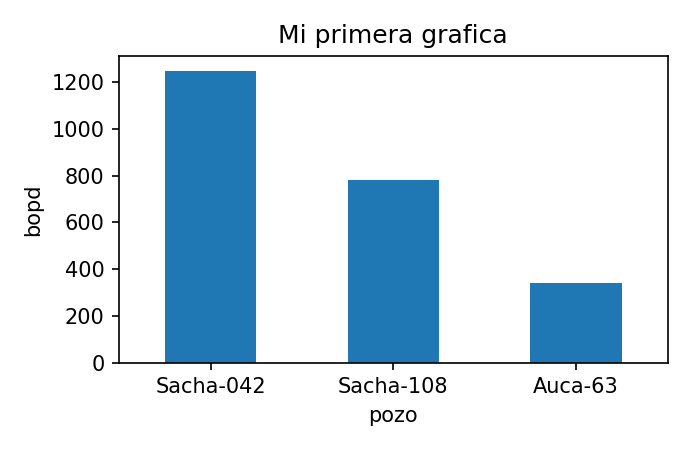
\includegraphics[width=0.82\textwidth]{fig_mini_bar.png}
    \end{column}
  \end{columns}
\end{frame}

% ─────────────────────────────────────────────────────────────────────────────
%  GRÁFICO 1: LÍNEA
% ─────────────────────────────────────────────────────────────────────────────
\begin{frame}[fragile,shrink=15]{Graficar con pandas: \texttt{.plot()}}
  \vspace{-4pt}
  {\small\color{arcaDark}\bfseries
    Ahora con datos de verdad: la producción del pozo F-12 contra el tiempo.}

  \vspace{4pt}
  \begin{columns}[T]
    \begin{column}{0.46\textwidth}
      \begin{pyblock}
prod["fecha"] = pd.to_datetime(
    prod["fecha"])

f12 = prod[prod["pozo"]
           == "15/9-F-12"]

f12.plot(x="fecha", y="oil")
      \end{pyblock}

      \vspace{4pt}
      {\scriptsize\color{textMuted}
      \begin{itemize}\setlength{\itemsep}{4pt}
        \item[{\color{arcaRed}\scriptsize\faArrowRight}]
          Detalle previo: \texttt{to\_datetime}
          convierte el \textbf{texto} del CSV en
          \textbf{fechas de verdad}, para que el
          eje X ordene bien.
        \item[{\color{arcaRed}\scriptsize\faArrowRight}]
          \texttt{.plot(x=..., y=...)}: qué columna
          va en cada eje. Y ya.
      \end{itemize}
      }
    \end{column}

    \begin{column}{0.52\textwidth}
      \centering
      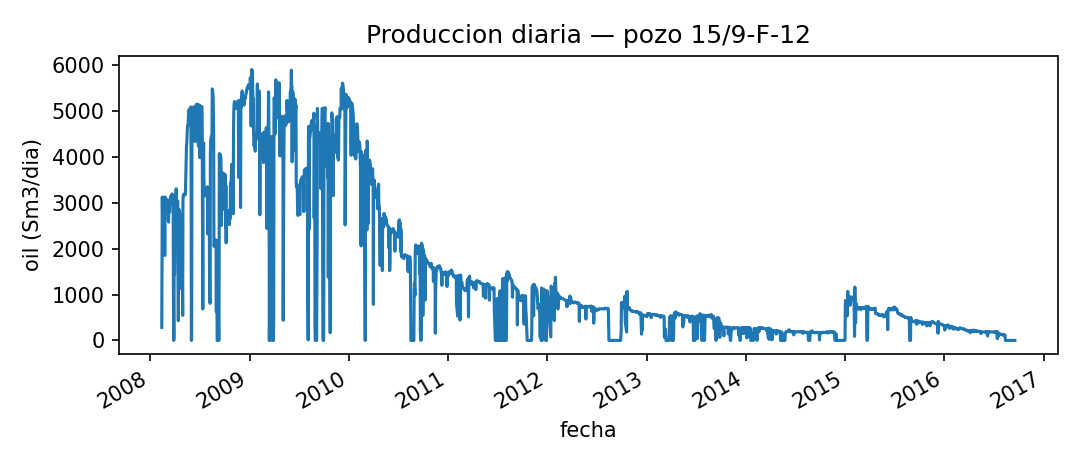
\includegraphics[width=\textwidth]{fig_prod_line.png}

      {\scriptsize\color{textMuted}\itshape
        La \textbf{curva de declive}: alta al inicio,
        cayendo con los años. Así viven y mueren los pozos.}
    \end{column}
  \end{columns}
\end{frame}

% ─────────────────────────────────────────────────────────────────────────────
%  GRÁFICO 2: BARRAS
% ─────────────────────────────────────────────────────────────────────────────
\begin{frame}[fragile,shrink=15]{Graficar un \texttt{groupby}: Barras}
  \vspace{-4pt}
  {\small\color{arcaDark}\bfseries
    El resumen por pozo, ahora como gráfico de barras.}

  \vspace{4pt}
  \begin{columns}[T]
    \begin{column}{0.46\textwidth}
      \begin{pyblock}
totales = (prod.groupby("pozo")
           ["oil"].sum())

totales.plot(kind="barh")
      \end{pyblock}

      \vspace{4pt}
      {\scriptsize\color{textMuted}
      \begin{itemize}\setlength{\itemsep}{4pt}
        \item[{\color{arcaRed}\scriptsize\faArrowRight}]
          \texttt{kind="barh"}: barras horizontales.
          (\texttt{"bar"} = verticales,
          \texttt{"line"} = línea).
        \item[{\color{codeGreen}\scriptsize\faCheck}]
          Dos pozos (F-12 y F-14) produjeron
          \textbf{el 85\%} de todo el campo.
      \end{itemize}
      }
    \end{column}

    \begin{column}{0.52\textwidth}
      \centering
      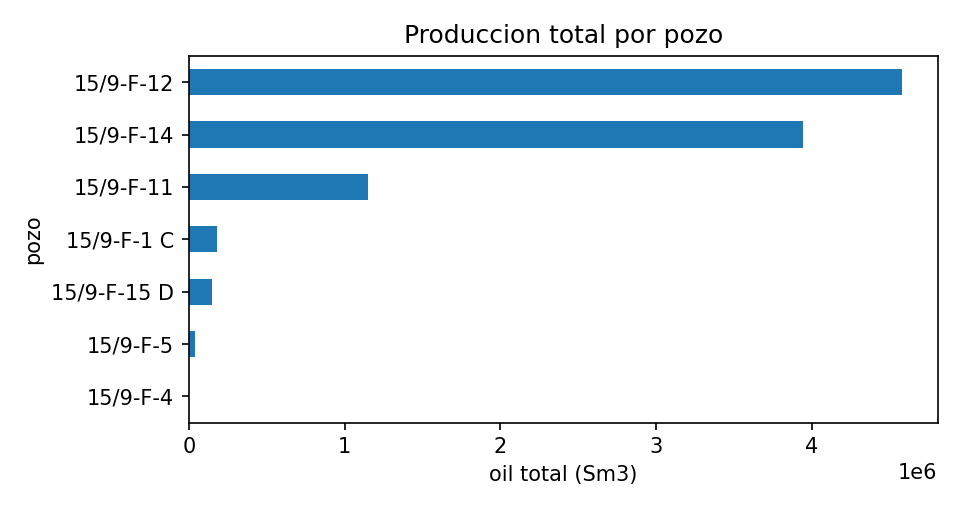
\includegraphics[width=\textwidth]{fig_pozos_barh.png}
    \end{column}
  \end{columns}
\end{frame}

% ─────────────────────────────────────────────────────────────────────────────
%  PRÁCTICA 4
% ─────────────────────────────────────────────────────────────────────────────
\begin{frame}[fragile,shrink=8]{Su Turno: Operar y Graficar \hfill {\normalsize\color{arcaRed}\faClock\hspace{4pt}10 min}}
  \vspace{-4pt}
  {\small\color{arcaDark}\bfseries
    Con la producción (\texttt{prod}) ya cargada:}

  \vspace{4pt}
  {\footnotesize
  \begin{enumerate}\setlength{\itemsep}{4pt}
    \item[{\color{arcaRed}\bfseries 1.}]
      ¿Cuál es la producción \textbf{promedio} de oil del campo? (\texttt{.mean()})
    \item[{\color{arcaRed}\bfseries 2.}]
      ¿Y el \textbf{describe} completo de la columna \texttt{gas}?
    \item[{\color{arcaRed}\bfseries 3.}]
      Filtrar los días del pozo \texttt{15/9-F-14} (\texttt{==}).
    \item[{\color{arcaRed}\bfseries 4.}]
      Graficar la producción de F-14 contra la fecha (\texttt{.plot(x=..., y=...)}).
    \item[{\color{arcaRed}\bfseries 5.}]
      Con \texttt{groupby}, calcular el \textbf{agua} total por pozo y graficarla en barras.
  \end{enumerate}
  }
\end{frame}

% ═════════════════════════════════════════════════════════════════════════════
\sectionframe{Well Logs y el Formato LAS}{El dato petrolero por excelencia}
% ═════════════════════════════════════════════════════════════════════════════

% ─────────────────────────────────────────────────────────────────────────────
%  ¿QUÉ ES UN WELL LOG?
% ─────────────────────────────────────────────────────────────────────────────
\begin{frame}{¿Qué es un Well Log (Registro de Pozo)?}
  \vspace{-6pt}
  {\small\color{arcaDark}\bfseries
    Al perforar, se baja una herramienta que mide las propiedades de la roca a lo largo del pozo.}

  \vspace{8pt}
  \begin{columns}[T]
    \begin{column}{0.48\textwidth}
      {\footnotesize\color{textMuted}
      \begin{itemize}\setlength{\itemsep}{6pt}
        \item[{\color{arcaRed}\scriptsize\faArrowDown}]
          El eje no es el tiempo: es la
          \textbf{profundidad} (metros).
        \item[{\color{arcaRed}\scriptsize\faChartLine}]
          Cada propiedad medida es una \textbf{curva}:
          radioactividad, densidad, resistividad\ldots
        \item[{\color{arcaRed}\scriptsize\faMicrochip}]
          La herramienta mide \textbf{cada pocos
          centímetros}: decenas de miles de registros
          por pozo.
      \end{itemize}
      }
    \end{column}

    \begin{column}{0.48\textwidth}
      {\footnotesize\color{arcaDark}\bfseries Las curvas responden preguntas:}
      \vspace{4pt}
      {\footnotesize\color{textMuted}
      \begin{itemize}\setlength{\itemsep}{6pt}
        \item[{\color{arcaRed}\scriptsize\faQuestion}]
          ¿Qué \textbf{tipo de roca} hay a cada
          profundidad? ¿Arena o arcilla?
        \item[{\color{arcaRed}\scriptsize\faQuestion}]
          ¿Tiene \textbf{poros} donde acumular
          petróleo?
        \item[{\color{arcaRed}\scriptsize\faQuestion}]
          Esos poros, ¿tienen \textbf{petróleo
          o agua}?
      \end{itemize}
      }
    \end{column}
  \end{columns}

  \vspace{8pt}
  \centering
  {\footnotesize\color{arcaDark}\itshape
    Es el dato con el que se decide dónde completar y producir un pozo.}
\end{frame}

% ─────────────────────────────────────────────────────────────────────────────
%  ¿QUÉ ES UN LAS?
% ─────────────────────────────────────────────────────────────────────────────
\begin{frame}[fragile,shrink=18]{El Formato LAS: el Estándar de la Industria}
  \vspace{-4pt}
  {\small\color{arcaDark}\bfseries
    LAS = \textit{Log ASCII Standard}. Desde 1990, todo software petrolero lo lee y lo escribe.}

  \vspace{4pt}
  \begin{columns}[T]
    \begin{column}{0.46\textwidth}
      {\scriptsize\color{textMuted}
      \begin{itemize}\setlength{\itemsep}{5pt}
        \item[{\color{arcaRed}\scriptsize\faFile}]
          Es \textbf{texto}, como el CSV, pero con
          una estructura propia.
        \item[{\color{arcaRed}\scriptsize\faInfoCircle}]
          Una \textbf{cabecera} describe el pozo:
          nombre, campo, operador, unidades\ldots
        \item[{\color{arcaRed}\scriptsize\faTable}]
          Después viene la \textbf{tabla de datos}:
          profundidad + una columna por curva.
        \item[{\color{arcaRed}\scriptsize\faIndustry}]
          Nuestro archivo: el pozo \textbf{15/9-19},
          perforado por \textbf{Statoil} (hoy Equinor).
      \end{itemize}
      }
    \end{column}

    \begin{column}{0.50\textwidth}
      \begin{outputblock}[title={\small\faFile\hspace{6pt}15-9-19.LAS (por dentro)}]
~Well Information
STRT.M   102.1568 : Top
STOP.M  4636.5140 : Bottom
STEP.M     .15240 : Increment
NULL.    -999.250 : Null Value
WELL.     15/9-19 : NAME
COMP.     STATOIL : OPERATOR
~Curve Information
DEPT.M    : DEPTH
GR  .GAPI : Gamma Ray
~ASCII
 102.15  -999.25  -999.25
 102.30  -999.25  -999.25
      \end{outputblock}
    \end{column}
  \end{columns}
\end{frame}

% ─────────────────────────────────────────────────────────────────────────────
%  LAS vs CSV
% ─────────────────────────────────────────────────────────────────────────────
\begin{frame}{LAS vs CSV: ¿En Qué se Diferencian?}
  \vspace{-6pt}
  {\small\color{arcaDark}\bfseries
    Los dos son texto y los dos son tablas. Pero cuentan cosas muy distintas.}

  \vspace{6pt}
  \centering
  {\footnotesize
  \renewcommand{\arraystretch}{1.45}
  \begin{tabular}{@{}p{3.2cm} p{4.1cm} p{4.3cm}@{}}
    \toprule
    & {\bfseries\color{arcaDark} CSV (producción)} & {\bfseries\color{arcaRed} LAS (well log)} \\
    \midrule
    {\bfseries Cada fila es\ldots} & un \textbf{día} de un pozo & una \textbf{profundidad} del pozo \\
    {\bfseries El ``eje'' es\ldots} & el tiempo (fechas) & la profundidad (metros) \\
    {\bfseries Espaciado} & un registro por día & un registro cada \textbf{15.24 cm} \\
    {\bfseries Metadatos} & ninguno (solo encabezado) & \textbf{cabecera completa}: pozo, operador, unidades \\
    {\bfseries Dato faltante} & celda vacía & código \texttt{-999.25} \\
    {\bfseries Quién lo usa} & cualquier industria & \textbf{estándar petrolero} \\
    \bottomrule
  \end{tabular}
  }

  \vspace{8pt}
  {\scriptsize\color{textMuted}
    \faLightbulb[regular]\hspace{3pt}%
    La buena noticia: una vez cargados en Python, \textbf{los dos se vuelven DataFrames} y se manejan igual.}
\end{frame}

% ─────────────────────────────────────────────────────────────────────────────
%  DIMENSIONES DEL LAS
% ─────────────────────────────────────────────────────────────────────────────
\begin{frame}[shrink=8]{Las Dimensiones del LAS: un Pozo en Números}
  \vspace{-6pt}
  {\small\color{arcaDark}\bfseries
    Nuestro archivo mide el pozo 15/9-19 desde 102 m hasta 4\,636 m de profundidad.}

  \vspace{4pt}
  \begin{columns}[T]
    \begin{column}{0.34\textwidth}
      \centering
      \begin{tikzpicture}[scale=0.9]
        % suelo
        \fill[arcaGray] (-1.7,0.25) rectangle (1.7,0.55);
        \draw[arcaLightGray, line width=0.5pt] (-1.7,0.25) -- (1.7,0.25);
        % torre
        \draw[arcaDark, line width=1pt] (-0.35,0.55) -- (0,1.35) -- (0.35,0.55);
        \draw[arcaDark, line width=0.7pt] (-0.22,0.85) -- (0.22,0.85);
        % pozo
        \fill[arcaRed!12] (-0.13,-4.3) rectangle (0.13,0.25);
        \draw[arcaRed, line width=1pt] (-0.13,0.25) -- (-0.13,-4.3);
        \draw[arcaRed, line width=1pt] (0.13,0.25) -- (0.13,-4.3);
        % marcas de profundidad
        \draw[textMuted, line width=0.5pt] (0.3,-0.15) -- (0.55,-0.15)
          node[right, font=\tiny\color{textMuted}] {102 m};
        \draw[textMuted, line width=0.5pt] (0.3,-4.15) -- (0.55,-4.15)
          node[right, font=\tiny\color{textMuted}] {4\,636 m};
        % zoom de paso
        \draw[arcaDark!60, line width=0.5pt] (-0.3,-2.0) -- (-0.85,-2.0);
        \draw[arcaDark!60, line width=0.5pt] (-0.3,-2.25) -- (-0.85,-2.25);
        \node[left, font=\tiny\color{arcaDark}, align=right] at (-0.85,-2.12)
          {una fila\\cada 15.24 cm};
      \end{tikzpicture}
    \end{column}

    \begin{column}{0.62\textwidth}
      \vspace{6pt}
      {\footnotesize
      \renewcommand{\arraystretch}{1.5}
      \begin{tabular}{@{}l l@{}}
        \toprule
        {\bfseries\color{arcaRed} Dimensión} & {\bfseries\color{arcaDark} Valor real del archivo} \\
        \midrule
        Profundidad inicial & 102.16 m \\
        Profundidad final   & 4\,636.51 m \\
        Paso de medición    & 0.1524 m (= 6 pulgadas) \\
        {\bfseries Filas (profundidades)} & {\bfseries 29\,754} \\
        {\bfseries Columnas (curvas)}     & {\bfseries 7} \\
        \bottomrule
      \end{tabular}
      }

      \vspace{8pt}
      {\scriptsize\color{textMuted}
      \begin{itemize}\setlength{\itemsep}{4pt}
        \item[{\color{arcaRed}\scriptsize\faArrowRight}]
          En el CSV el índice era 0, 1, 2\ldots
          Aquí el índice \textbf{es la profundidad}.
        \item[{\color{arcaRed}\scriptsize\faArrowRight}]
          29\,754 filas \(\times\) 7 curvas
          \(\approx\) \textbf{208 mil mediciones} en un solo pozo.
      \end{itemize}
      }
    \end{column}
  \end{columns}
\end{frame}

% ─────────────────────────────────────────────────────────────────────────────
%  LAS CURVAS: QUÉ MIDE CADA UNA
% ─────────────────────────────────────────────────────────────────────────────
\begin{frame}[shrink=10]{Las 7 Curvas: Qué nos Dice Cada Columna}
  \vspace{-6pt}
  {\small\color{arcaDark}\bfseries
    Cada columna del LAS es un ``sensor'' distinto de la roca. Estas son las del pozo 15/9-19:}

  \vspace{5pt}
  \centering
  {\footnotesize
  \renewcommand{\arraystretch}{1.4}
  \begin{tabular}{@{}l l l l@{}}
    \toprule
    {\bfseries\color{arcaRed} Curva} & {\bfseries\color{arcaDark} Unidad}
      & {\bfseries\color{arcaDark} Qué mide} & {\bfseries\color{arcaDark} Qué nos dice} \\
    \midrule
    \texttt{GR}   & GAPI  & radioactividad natural & arcilla (alta) vs arena (baja) \\
    \texttt{DEN}  & g/cm\(^3\) & densidad de la roca & porosidad \\
    \texttt{NEU}  & \%    & respuesta al neutrón & porosidad (hidrógeno) \\
    \texttt{AC}   & \(\mu\)s/ft & velocidad del sonido & porosidad, dureza \\
    \texttt{RDEP} & ohm\(\cdot\)m & resistividad profunda & \textbf{¿petróleo o agua?} \\
    \texttt{RMED} & ohm\(\cdot\)m & resistividad media & compara con RDEP \\
    \texttt{CALI} & pulgadas & diámetro del hueco & calidad de la medición \\
    \bottomrule
  \end{tabular}
  }

  \vspace{8pt}
  {\scriptsize\color{textMuted}
    \faLightbulb[regular]\hspace{3pt}%
    La clave de la resistividad: el agua salada \textbf{conduce} electricidad (resistividad baja);
    el petróleo \textbf{no conduce} (alta). Un RDEP alto en roca porosa = zona de interés.}
\end{frame}

% ─────────────────────────────────────────────────────────────────────────────
%  LASIO
% ─────────────────────────────────────────────────────────────────────────────
\begin{frame}[fragile,shrink=15]{lasio: la Librería para Leer LAS}
  \vspace{-4pt}
  {\small\color{arcaDark}\bfseries
    Los tres pasos de toda librería: instalar \(\to\) importar \(\to\) usar.}

  \vspace{4pt}
  \begin{columns}[T]
    \begin{column}{0.52\textwidth}
      \begin{pyblock}
!pip install lasio

import lasio

las = lasio.read(url_las)
log = las.df()   # a DataFrame

print(log.shape)
print(list(log.columns))
      \end{pyblock}
    \end{column}

    \begin{column}{0.44\textwidth}
      \begin{outputblock}
(29754, 7)
['AC', 'CALI', 'DEN', 'GR',
 'NEU', 'RDEP', 'RMED']
      \end{outputblock}

      \vspace{4pt}
      {\scriptsize\color{textMuted}
      \begin{itemize}\setlength{\itemsep}{4pt}
        \item[{\color{arcaRed}\scriptsize\faArrowRight}]
          \texttt{lasio} \textbf{no viene} en Colab:
          por eso el \texttt{pip install}.
        \item[{\color{arcaRed}\scriptsize\faArrowRight}]
          \texttt{.df()} convierte el LAS en un
          \textbf{DataFrame}: cabecera afuera,
          curvas adentro.
        \item[{\color{codeGreen}\scriptsize\faCheck}]
          Los \texttt{-999.25} se vuelven
          \texttt{NaN} automáticamente.
      \end{itemize}
      }
    \end{column}
  \end{columns}
\end{frame}

% ─────────────────────────────────────────────────────────────────────────────
%  GRÁFICO 3: CURVA GR
% ─────────────────────────────────────────────────────────────────────────────
\begin{frame}[fragile,shrink=15]{Graficar una Curva del Well Log}
  \vspace{-4pt}
  {\small\color{arcaDark}\bfseries
    En el log, el índice es la profundidad: \texttt{.plot()} la pone automáticamente en el eje X.}

  \vspace{4pt}
  \begin{columns}[T]
    \begin{column}{0.46\textwidth}
      \begin{pyblock}
log["GR"].plot()
      \end{pyblock}

      \vspace{4pt}
      {\scriptsize\color{textMuted}
      \begin{itemize}\setlength{\itemsep}{4pt}
        \item[{\color{arcaRed}\scriptsize\faArrowRight}]
          Una sola línea: la Series \texttt{GR}
          contra su índice (la profundidad).
        \item[{\color{arcaRed}\scriptsize\faArrowRight}]
          Los picos de GR = zonas con más
          \textbf{arcilla}; los valles = \textbf{arenas}
          (posibles reservorios).
        \item[{\color{arcaRed}\scriptsize\faInfoCircle}]
          Los petrofísicos lo dibujan en
          \textbf{vertical}; lo aprenderemos
          más adelante en el diplomado.
      \end{itemize}
      }
    \end{column}

    \begin{column}{0.52\textwidth}
      \centering
      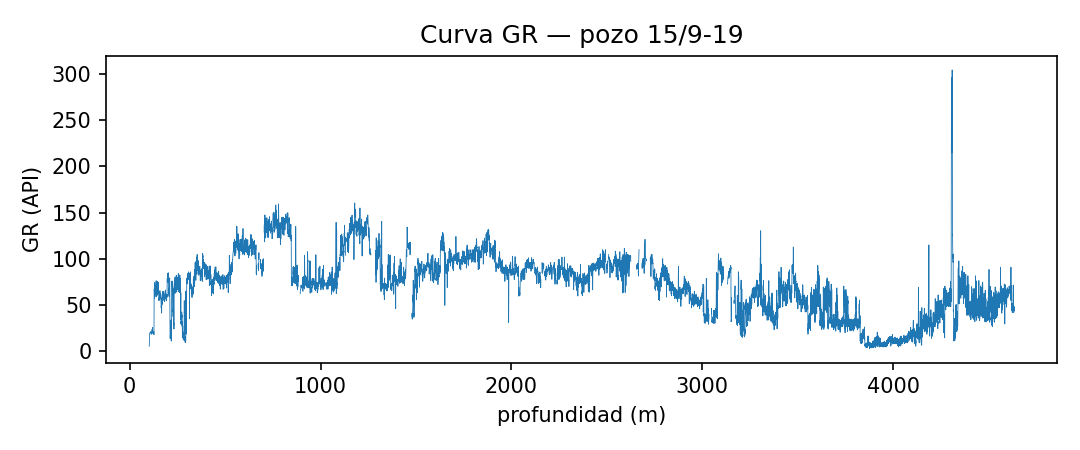
\includegraphics[width=\textwidth]{fig_gr_line.png}
    \end{column}
  \end{columns}
\end{frame}

% ─────────────────────────────────────────────────────────────────────────────
%  PRÁCTICA 3
% ─────────────────────────────────────────────────────────────────────────────
\begin{frame}[fragile,shrink=8]{Su Turno: Abrir el Well Log \hfill {\normalsize\color{arcaRed}\faClock\hspace{4pt}7 min}}
  \vspace{-4pt}
  {\small\color{arcaDark}\bfseries
    Lean el LAS del pozo 15/9-19 y explórenlo como DataFrame.}

  \vspace{4pt}
  {\footnotesize\color{textMuted}En el notebook:}

  \vspace{2pt}
  {\footnotesize
  \begin{enumerate}\setlength{\itemsep}{4pt}
    \item[{\color{arcaRed}\bfseries 1.}]
      Instalar \texttt{lasio} con \texttt{!pip install lasio}.
    \item[{\color{arcaRed}\bfseries 2.}]
      Importarlo y leer el archivo desde la URL con \texttt{lasio.read(...)}.
    \item[{\color{arcaRed}\bfseries 3.}]
      Convertirlo a DataFrame con \texttt{.df()}.
    \item[{\color{arcaRed}\bfseries 4.}]
      ¿Cuántas filas tiene? ¿Qué curvas trae? (\texttt{.shape}, \texttt{.columns})
    \item[{\color{arcaRed}\bfseries 5.}]
      Ver \texttt{.head()}: ¿por qué hay tantos \texttt{NaN} al inicio?
    \item[{\color{arcaRed}\bfseries 6.}]
      Sacar el \texttt{.describe()} de la curva \texttt{GR} y \textbf{graficarla} con \texttt{.plot()}.
  \end{enumerate}
  }

  \vspace{3pt}
  {\scriptsize\color{textMuted}\itshape
    \faLightbulb[regular]\hspace{3pt}%
    Pista de la 5: las herramientas no miden desde la superficie; cada curva cubre solo un tramo del pozo.}
\end{frame}

% ═════════════════════════════════════════════════════════════════════════════
\sectionframe{Limpieza de Datos}{Breve pero esencial}
% ═════════════════════════════════════════════════════════════════════════════

% ─────────────────────────────────────────────────────────────────────────────
%  NAN: DETECTAR
% ─────────────────────────────────────────────────────────────────────────────
\begin{frame}[fragile,shrink=15]{Datos Faltantes: Contarlos Primero}
  \vspace{-4pt}
  {\small\color{arcaDark}\bfseries
    Ya vimos los \texttt{NaN}. El primer paso siempre es saber \textbf{cuántos hay y dónde}.}

  \vspace{4pt}
  \begin{columns}[T]
    \begin{column}{0.50\textwidth}
      \begin{pyblock}
prod.isna().sum()
      \end{pyblock}
      \vspace{2pt}
      \begin{outputblock}
fecha       0
pozo        0
horas     285
oil      6473
gas      6473
agua     6473
      \end{outputblock}
    \end{column}

    \begin{column}{0.46\textwidth}
      {\scriptsize\color{textMuted}
      \begin{itemize}\setlength{\itemsep}{5pt}
        \item[{\color{arcaRed}\scriptsize\faArrowRight}]
          \texttt{.isna()} marca cada celda vacía;
          \texttt{.sum()} las cuenta por columna.
        \item[{\color{arcaRed}\scriptsize\faArrowRight}]
          \textbf{6\,473} días sin producción registrada
          (de 15\,634): pozos aún no perforados
          o cerrados.
        \item[{\color{codeGreen}\scriptsize\faCheck}]
          Es \textbf{normal} en datos reales.
          Lo importante es decidir qué hacer.
      \end{itemize}
      }
    \end{column}
  \end{columns}
\end{frame}

% ─────────────────────────────────────────────────────────────────────────────
%  DROPNA / FILLNA
% ─────────────────────────────────────────────────────────────────────────────
\begin{frame}[fragile,shrink=15]{Dos Remedios: Borrar o Rellenar}
  \vspace{-4pt}
  {\small\color{arcaDark}\bfseries
    \texttt{dropna()} elimina las filas con huecos; \texttt{fillna()} los completa con un valor.}

  \vspace{4pt}
  \begin{columns}[T]
    \begin{column}{0.48\textwidth}
      {\scriptsize\color{arcaRed}\bfseries\faTrash\hspace{3pt}Borrar (con cuidado)}
      \begin{pyblock}
limpio = prod.dropna()
print(prod.shape)
print(limpio.shape)
      \end{pyblock}
      \vspace{2pt}
      \begin{outputblock}
(15634, 7)
(9161, 7)
      \end{outputblock}
    \end{column}

    \begin{column}{0.48\textwidth}
      {\scriptsize\color{codeGreen}\bfseries\faPlus\hspace{3pt}Rellenar (aquí, con 0)}
      \begin{pyblock}
prod["oil"] = prod["oil"].fillna(0)
prod["agua"] = prod["agua"].fillna(0)
      \end{pyblock}
      \vspace{4pt}
      {\scriptsize\color{textMuted}
        Pozo cerrado = 0 producción: aquí
        rellenar con 0 \textbf{tiene sentido físico}.
        En otros datos podría ser el promedio,
        o interpolar entre vecinos
        (\texttt{.interpolate()}, útil en logs).}
    \end{column}
  \end{columns}

  \vspace{5pt}
  {\scriptsize\color{textMuted}
    \faLightbulb[regular]\hspace{3pt}%
    No hay receta única: borrar bota información; rellenar inventa valores. La decisión depende
    de \textbf{qué significa} el hueco.}
\end{frame}

% ─────────────────────────────────────────────────────────────────────────────
%  PRÁCTICA INTEGRADORA
% ─────────────────────────────────────────────────────────────────────────────
\begin{frame}[fragile,shrink=8]{Práctica Integradora: Reporte Volve \hfill {\normalsize\color{arcaRed}\faClock\hspace{4pt}15 min}}
  \vspace{-4pt}
  {\small\color{arcaDark}\bfseries
    Todo lo de hoy, junto: el mismo reporte de la Clase 2, ahora con 15\,634 filas reales.}

  \vspace{4pt}
  {\footnotesize
  \begin{enumerate}\setlength{\itemsep}{4pt}
    \item[{\color{arcaRed}\bfseries 1.}]
      \textbf{Cargar} el CSV de producción desde la URL.
    \item[{\color{arcaRed}\bfseries 2.}]
      \textbf{Contar} los faltantes por columna con \texttt{.isna().sum()}.
    \item[{\color{arcaRed}\bfseries 3.}]
      \textbf{Rellenar} con 0 los \texttt{NaN} de \texttt{oil}, \texttt{gas} y \texttt{agua}.
    \item[{\color{arcaRed}\bfseries 4.}]
      \textbf{Convertir} \texttt{fecha} con \texttt{pd.to\_datetime}.
    \item[{\color{arcaRed}\bfseries 5.}]
      \textbf{Resumir}: producción total de oil por pozo (\texttt{groupby}). ¿Cuál produjo más?
    \item[{\color{arcaRed}\bfseries 6.}]
      \textbf{Graficar}: la producción del mejor pozo contra la fecha, y los totales en barras.
  \end{enumerate}
  }

  \vspace{4pt}
  {\scriptsize\color{textMuted}\itshape
    En la Clase 2, el reporte de 5 pozos nos tomó \(\sim\)25 líneas.
    Hoy, con 15\,634 filas, son \(\sim\)8.}
\end{frame}

% ═════════════════════════════════════════════════════════════════════════════
\sectionframe{Cierre}{Recapitulación}
% ═════════════════════════════════════════════════════════════════════════════

% ─────────────────────────────────────────────────────────────────────────────
%  RECAP
% ─────────────────────────────────────────────────────────────────────────────
\begin{frame}{Lo Que Aprendimos Hoy}
  \vspace{-6pt}
  \begin{columns}[T]
    \begin{column}{0.48\textwidth}
      {\footnotesize\color{arcaDark}\bfseries Conceptos}
      \vspace{3pt}
      {\footnotesize\color{textMuted}
      \begin{itemize}\setlength{\itemsep}{2pt}
        \item[{\color{codeGreen}\scriptsize\faCheck}]
          Dato, dataset y datos tabulares
        \item[{\color{codeGreen}\scriptsize\faCheck}]
          Qué es una librería; \texttt{pip} e \texttt{import}
        \item[{\color{codeGreen}\scriptsize\faCheck}]
          Diccionarios: \texttt{\{clave: valor\}}
        \item[{\color{codeGreen}\scriptsize\faCheck}]
          DataFrame y Series (pandas)
        \item[{\color{codeGreen}\scriptsize\faCheck}]
          Qué es un well log y el formato \textbf{LAS}
        \item[{\color{codeGreen}\scriptsize\faCheck}]
          Qué mide cada curva (GR, DEN, RDEP\ldots)
        \item[{\color{codeGreen}\scriptsize\faCheck}]
          Qué es un \texttt{NaN} y de dónde sale
      \end{itemize}
      }
    \end{column}

    \begin{column}{0.48\textwidth}
      {\footnotesize\color{arcaDark}\bfseries Habilidades}
      \vspace{3pt}
      {\footnotesize\color{textMuted}
      \begin{itemize}\setlength{\itemsep}{2pt}
        \item[{\color{codeGreen}\scriptsize\faCheck}]
          Cargar CSV por URL, subida o Drive
        \item[{\color{codeGreen}\scriptsize\faCheck}]
          Leer un LAS con \texttt{lasio}
        \item[{\color{codeGreen}\scriptsize\faCheck}]
          \texttt{head}, \texttt{shape}, \texttt{describe}, \texttt{unique}
        \item[{\color{codeGreen}\scriptsize\faCheck}]
          Filtrar filas y crear columnas
        \item[{\color{codeGreen}\scriptsize\faCheck}]
          Resumir con \texttt{groupby}
        \item[{\color{codeGreen}\scriptsize\faCheck}]
          Graficar con \texttt{.plot()} (línea y barras)
        \item[{\color{codeGreen}\scriptsize\faCheck}]
          Limpiar con \texttt{dropna} / \texttt{fillna}
      \end{itemize}
      }
    \end{column}
  \end{columns}

  \vspace{6pt}
  \centering
  {\footnotesize\color{arcaDark}
    \textbf{Habilidad clave:} tomar un archivo real, cargarlo, limpiarlo y sacar conclusiones.}
\end{frame}

% ─────────────────────────────────────────────────────────────────────────────
%  CIERRE DEL BLOQUE
% ─────────────────────────────────────────────────────────────────────────────
\begin{frame}{Cierre del Bloque de Python}
  \vspace{-6pt}
  {\small\color{arcaDark}\bfseries
    En 3 clases pasamos de cero a analizar datos petroleros reales.}

  \vspace{10pt}
  {\footnotesize
  \begin{itemize}\setlength{\itemsep}{8pt}
    \item[{\color{arcaRed}\Large\faArrowCircleRight}]
      \textbf{Clase 1} --- Fundamentos: variables, tipos, \texttt{input}, primeras decisiones.

    \item[{\color{arcaRed}\Large\faArrowCircleRight}]
      \textbf{Clase 2} --- Control de flujo: \texttt{if/elif/else}, listas, ciclos \texttt{for}.

    \item[{\color{arcaRed}\Large\faArrowCircleRight}]
      \textbf{Clase 3} --- pandas: librerías, carga de archivos reales (CSV y LAS),
      operaciones, gráficos y limpieza.

    \item[{\color{arcaRed}\Large\faArrowCircleRight}]
      \textbf{Lo que sigue} --- profundizar el análisis y llegar a los
      \textbf{modelos predictivos} sobre estos mismos datos.
  \end{itemize}
  }

  \vspace{8pt}
  \centering
  {\footnotesize\color{textMuted}\itshape
    Ya pueden dirigir y auditar un análisis de datos: cargar, limpiar, resumir y graficar.}
\end{frame}

% ─────────────────────────────────────────────────────────────────────────────
%  GRACIAS
% ─────────────────────────────────────────────────────────────────────────────
\begingroup
\setbeamertemplate{headline}{}
\setbeamertemplate{footline}{}
\setbeamertemplate{navigation symbols}{}
\begin{frame}[plain, noframenumbering]
  \begin{tikzpicture}[remember picture, overlay]
    \fill[arcaDark] (current page.south west) rectangle (current page.north east);
    \node[anchor=center, text=white, font=\Huge\bfseries]
      at ([yshift=1.5cm]current page.center) {¡Gracias!};
    \node[anchor=center, text=white!80, font=\large, text width=10cm, align=center]
      at ([yshift=0.2cm]current page.center)
      {Carlos Enrique Mosquera Trujillo};
    \node[anchor=center, text=white!60, font=\normalsize, text width=10cm, align=center]
      at ([yshift=-0.6cm]current page.center)
      {\faEnvelope\hspace{6pt}cmosquerat@unal.edu.co};
    \node[anchor=center, text=white!60, font=\normalsize, text width=10cm, align=center]
      at ([yshift=-1.3cm]current page.center)
      {Diplomado en Data Science Aplicada con Python};
    \node[anchor=center, text=white!40, font=\small]
      at ([yshift=-2.0cm]current page.center)
      {SLB Ecuador \quad$\cdot$\quad UDLA \quad$\cdot$\quad 2026};
  \end{tikzpicture}
\end{frame}
\endgroup

\end{document}
